\noindent
In this Section the user interface design, already presented in  \textit{Section 3.1.1 User Interfaces} of \textit{Requirements and Analysis Specification Document} with several mockups, is explained in more detail. A special attention is focused on the interaction between the user and the systems, and how the mockups are correlated each other.
\bigbreak
\noindent
\begin{enumerate}
\item[•]{\Large Data4Help}
\bigbreak
\noindent
Third parties can interact with Data4Help system through a Website which what they can made the several kind of requests.
\begin{figure}[H]
        \centering
          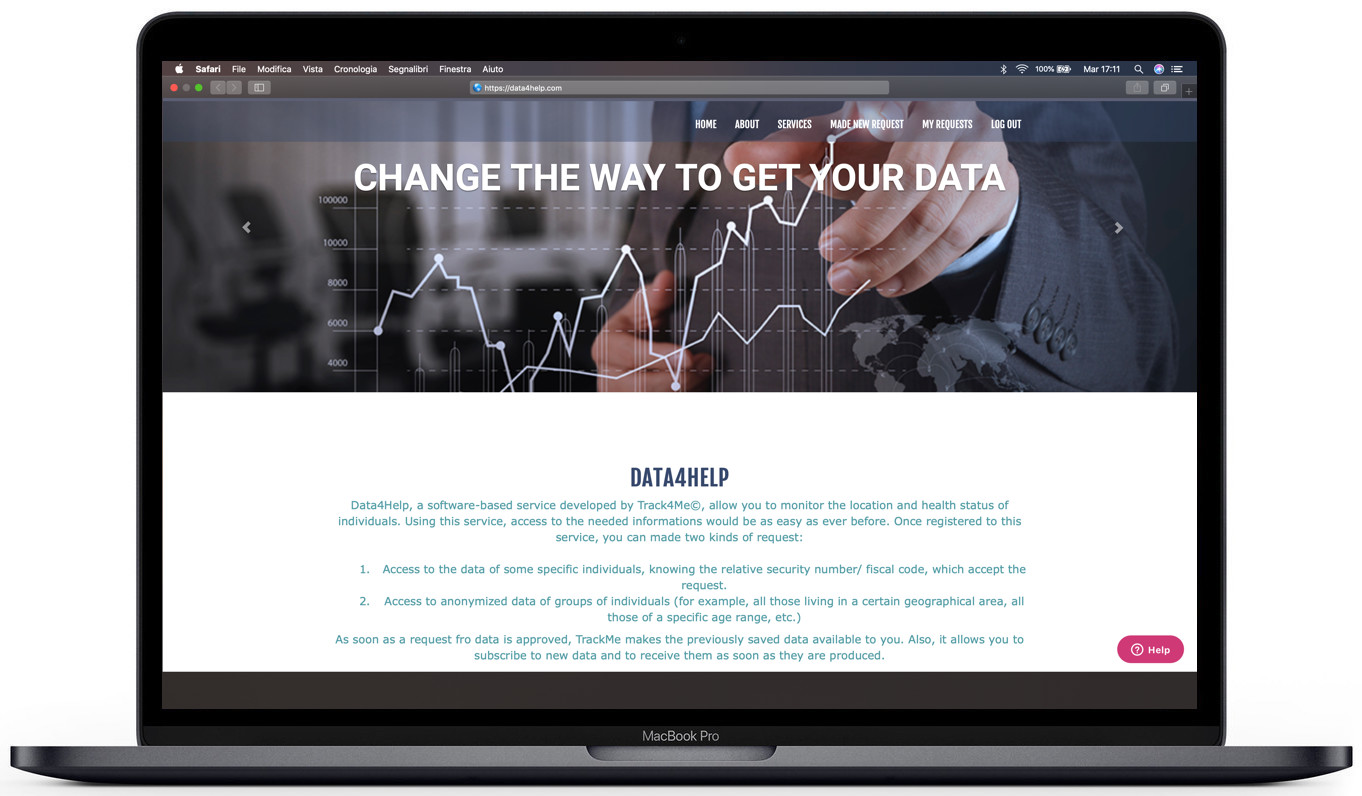
\includegraphics[scale = 0.33]{Images/Mockups/Homepage.jpg}
          	\caption{Data4Help's homepage}
\end{figure}
This is the homepage of Data4Help's website, reachable from the user's browser by the link \textit{www.data4help.com}. In the homepage it's possible to read a brief overviwe of the service offerd by Track4Me. Several actions are possible from here click on the different buttons present in the head \textbf{HOME}, \textbf{ABOUT}, \textbf{SERVICES}, \textbf{MADE NEW REQUEST}, and since the user is already logged into thesystem also the options \textbf{MY REQUESTS} and \textbf{LOG OUT} are available.Besides the options selectable into the header, scrolling down the page it is possible to select a button to directly made a monitoring request. 
\bigbreak
\noindent
Clicking on \textbf{MY REQUESTS} a list of all the historical requests will appear, both the approved, the denied and those waiting for the approbation. For the approved ones it is also possible to see the relative answers containing all the request informations.
\clearpage

\begin{figure}[H]
        \centering
          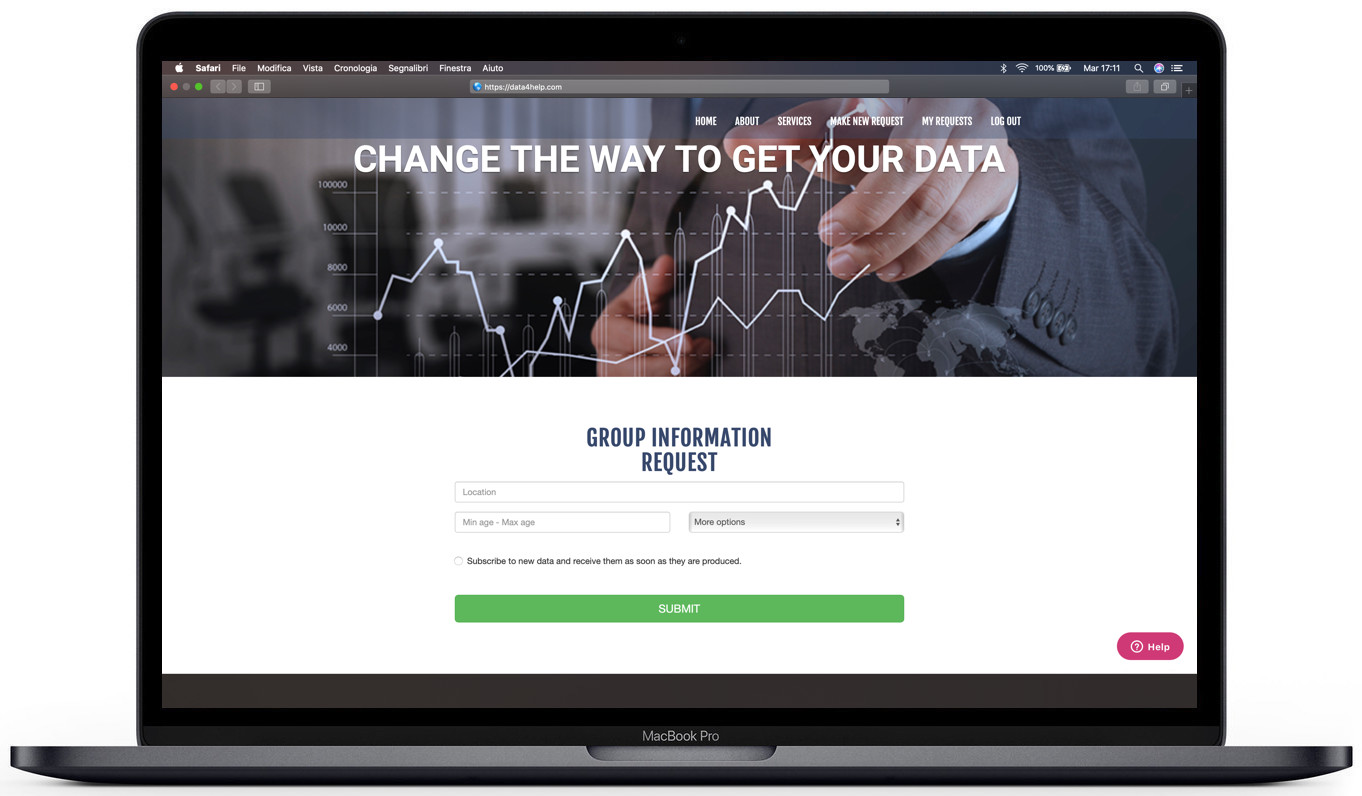
\includegraphics[scale = 0.33]{Images/Mockups/IndividualRequest.jpg}
          	\caption{Individual request form}
\end{figure}
Clicking on \textbf{MADE NEW REQUEST}, the Website loads another page where the third party is asked to select an option between \textbf{INDIVIDUAL MONITORING REQUEST} and \textbf{GROUP MONITORING REQUEST}. Clicking on the first option the system loads a new page containing the form to made a individual monitoring request. Once filled the security number's field it is possible to submit the request pressing the \textbf{SUBMIT} button.
\clearpage

\begin{figure}[H]
        \centering
          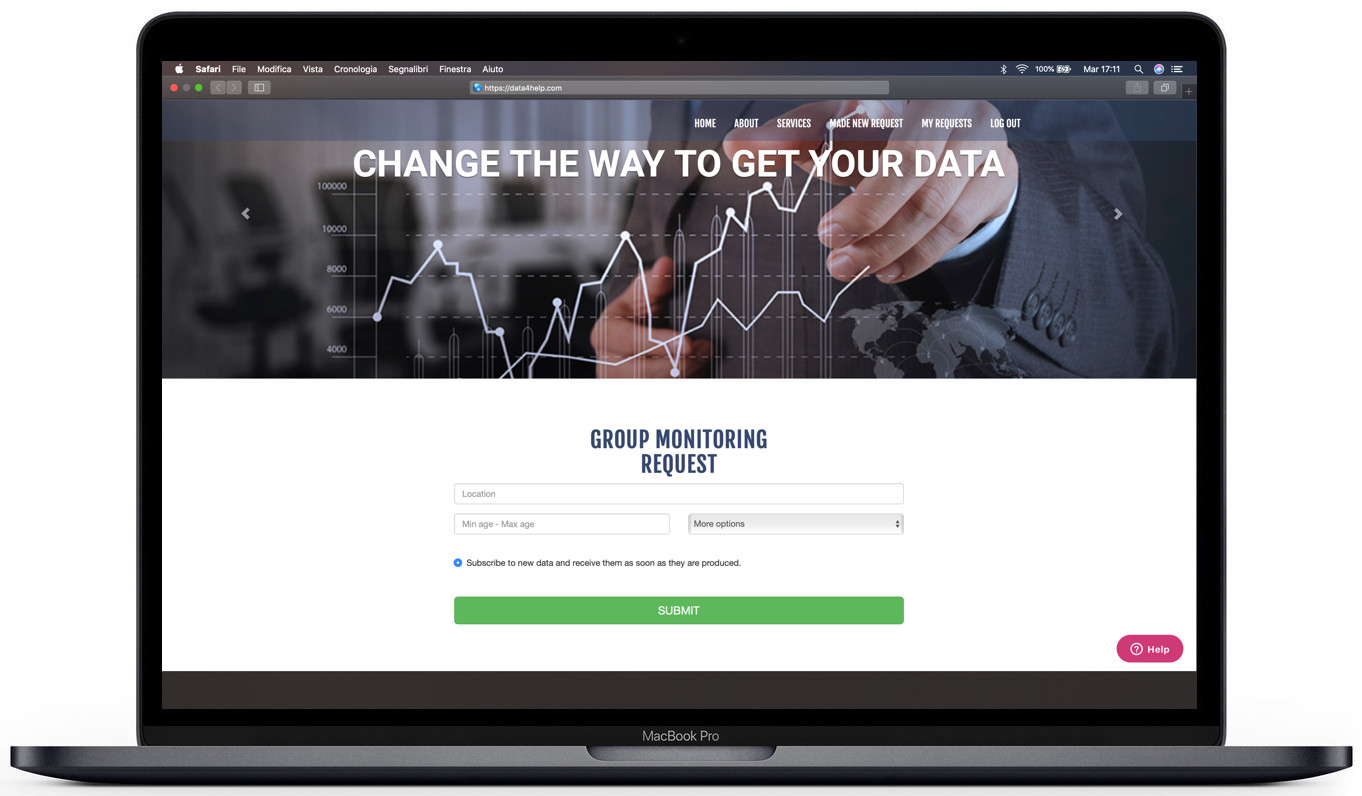
\includegraphics[scale = 0.33]{Images/Mockups/GroupRequest.jpg}
          	\caption{Group request form}
\end{figure}
Otherwise, clicking on \textbf{GROUP MONITORING REQUEST} button the system loads a new page containing the form to made a group monitoring request. In the form it is possible to limit the request to a group living in a specific zone, writing the geographical area on the \textbf{Location} field. It's then possible to select a minimum and a maximum age. Click one the \textbf{More options} button it's possible to limit furthermore the request adding other filters to the group of individuals. Once the user has fill al the fields, clicking on the \textbf{SUBMIT} button the request is forward to Data4Help system.
\clearpage

\item[•]{\Large AutomatedSOS}
\bigbreak
\noindent
TrackMe offers to AutomatedSOS users an App for smartwatches, with which the users can see their location and health status information.
\begin{figure}[H]
\begin{center}
        \begin{minipage}[c]{.40\textwidth}
        \centering
          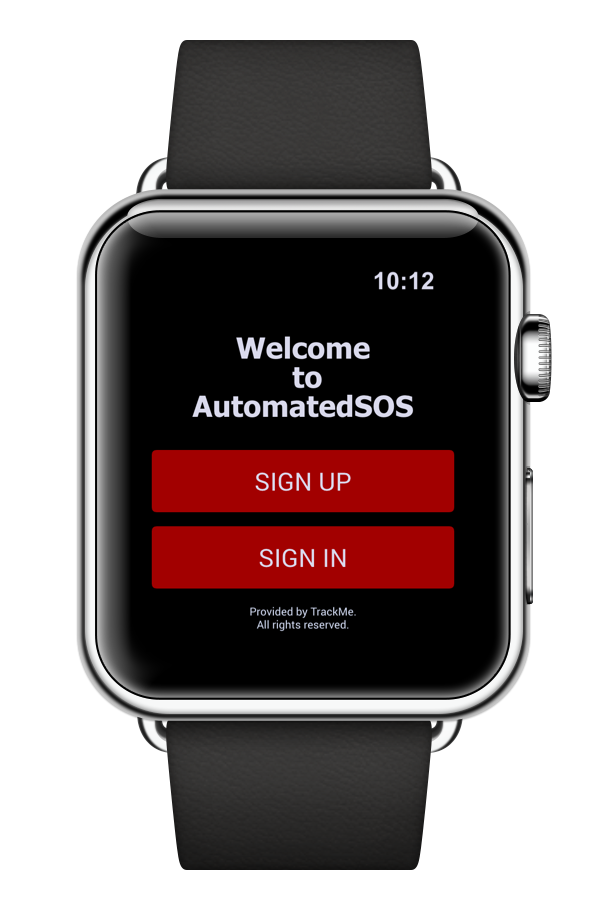
\includegraphics[height=12 cm]{Images/Mockups/AutomatedSOSMockup1.png}
          	\caption{Welcome page.}
        \end{minipage}%
        \hspace{10mm}%
        \begin{minipage}[c]{.40\textwidth}
        \centering
          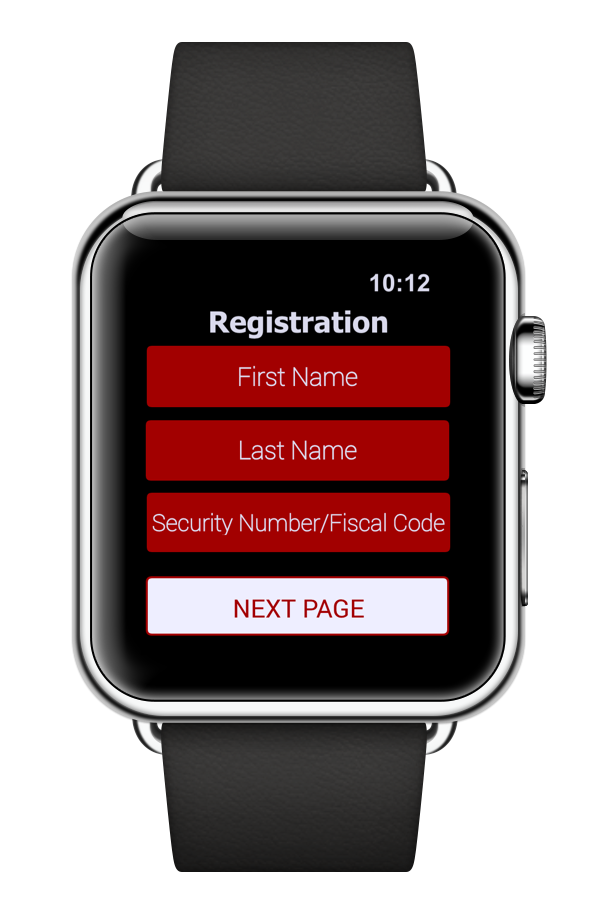
\includegraphics[height=12 cm]{Images/Mockups/AutomatedSOSMockup6.png}
          	\caption{Registration form.}
        \end{minipage}
      \end{center}
\end{figure}
In the first access to AutomatedSOS App the user is asked to sign up or to sign in 			(Figure 2). Based on the fact that the user already has a TrackMe account or not will choose the right option. In future accesses to the App the user do not need to select each time one of these two possible options because the App automatically remembers the account which is logged in. In case of sign in (Figure 3), the user has to fill all the mandatory fields in order to complete the registration form. Scrolling down the screen other fields will appear. Once every field is correctly filled, it would be possible to select the \textbf{NEXT PAGE} button. 
\clearpage
\begin{figure}[H]
\begin{center}
        \begin{minipage}[c]{.40\textwidth}
        \centering
          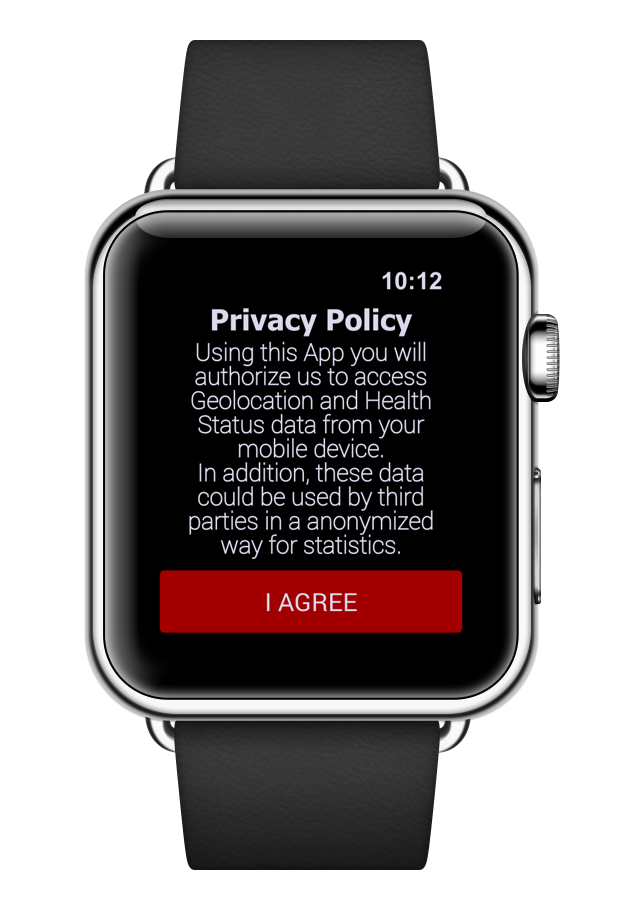
\includegraphics[height=12 cm]{Images/Mockups/AutomatedSOSMockup2.png}
             	\caption{Privacy Policy Conditions.}
        \end{minipage}%
        \hspace{10mm}%
        \begin{minipage}[c]{.40\textwidth}
        \centering
          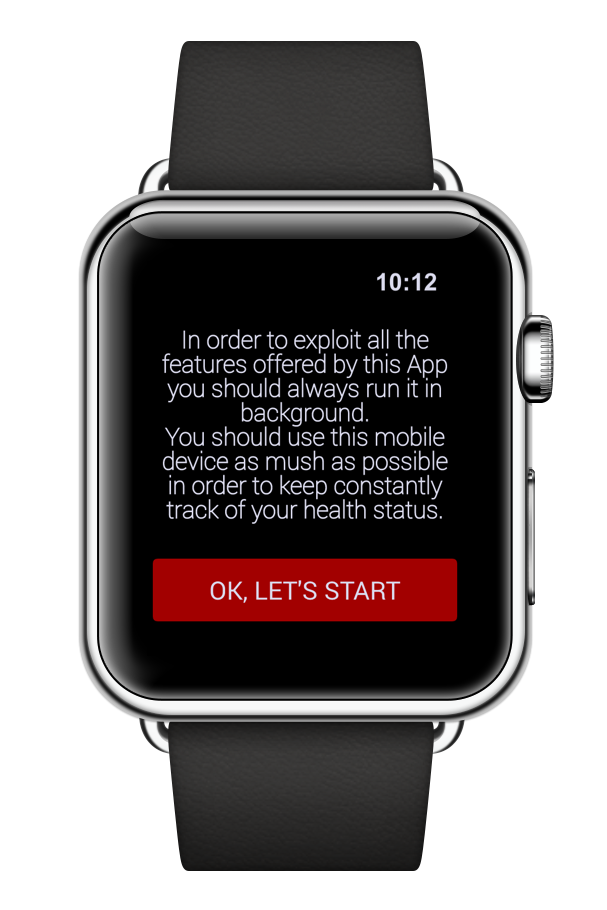
\includegraphics[height=12 cm]{Images/Mockups/AutomatedSOSMockup4.png}
          	\caption{Usage Conditions.}
        \end{minipage}
      \end{center}
\end{figure}
During the first access to the App, the next step after sign up/sign in is to agree to the Privacy Policy Conditions (Figure 4). In order to use this App the user has to agree to the treatment of Location and Health Status data by Data4Help. In addition, these data could be used by third parties for the group monitoring request. Without agreeing the Privacy Policy Conditions the user cannot go to the next page, therefore he/she will not be able to use this App. The last step before starting use the App is taking note of the importance of wearing the Smartwatch as much as possible and to let the App runs in background (Figure 5).
\clearpage
\begin{figure}
\begin{center}
	\bigbreak
        \begin{minipage}[c]{.40\textwidth}
        \centering
          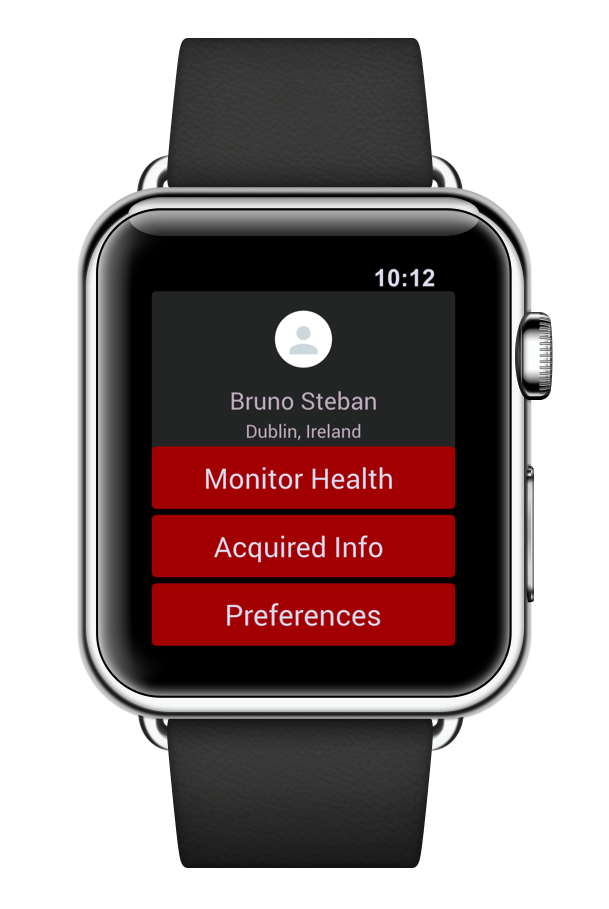
\includegraphics[height=12 cm]{Images/Mockups/AutomatedSOSMockup5.png}
          	\caption{Main menu.}
        \end{minipage}%
        \hspace{10mm}%
        \begin{minipage}[c]{.40\textwidth}
        \centering
          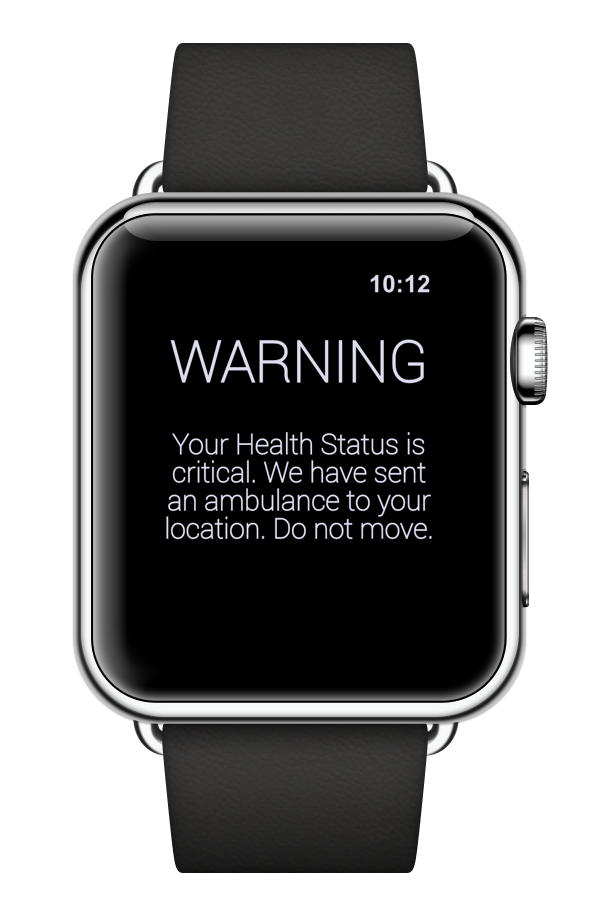
\includegraphics[height=12 cm]{Images/Mockups/AutomatedSOSMockup7.png}
          	\caption{Warning message.}
        \end{minipage}
      \end{center}
\end{figure}
The main menu of the App, which is immediately accessible by selecting the AutomatedSOS App on the Smartwatch home, is composed by three parts (Figure 6). Selecting \textbf{Monitor Health} the user can see live health informations, like the current Heart Rate, Blood Pressure and so on. Choosing the \textbf{Acquired Info} button the user can see all the historical data stored since the first access to the App. Finally, \textbf{Preferences} option allow to the user to set own threshold parameters according to the particular illnesses he/she is affected, own age and so on. As soon as an ambulance request is done due to the user's critical health status a warning message (Figure 7) appears on the screen of the Smartwatch notified by an alert sound.
\clearpage

\item[•]{\Large Track4Run}
\bigbreak
\noindent
Track4Run users can use an App for smartphone and another one for smartwatches. The first one could be used by everyone, while the second one is made only for the athletes.
\\[0.5 cm]
\begin{figure}[H]
\begin{center}
        \begin{minipage}[c]{.40\textwidth}
        \centering
          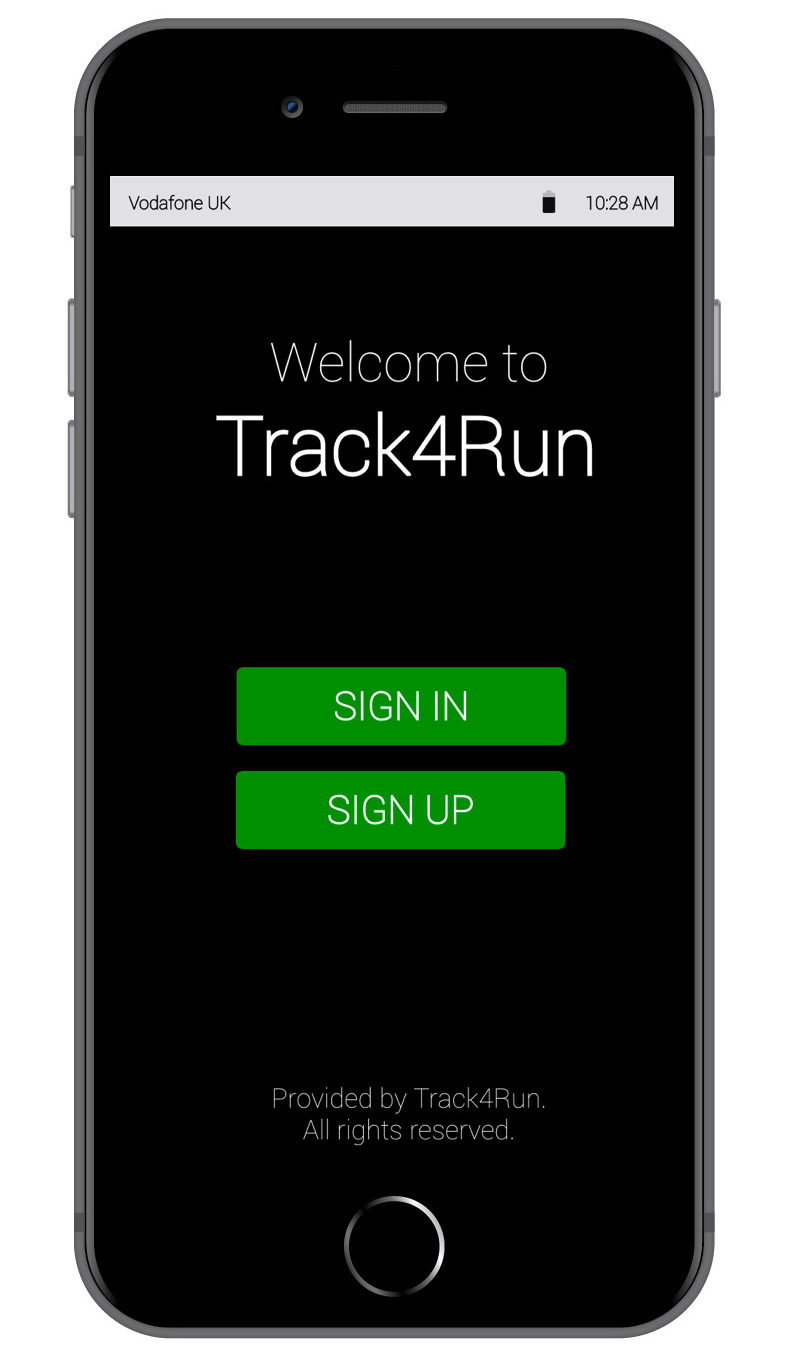
\includegraphics[height=14 cm]{Images/Mockups/Track4RunMockup1.jpg}
	\caption{Welcome page. }
        \end{minipage}%
        \hspace{10mm}%
        \begin{minipage}[c]{.40\textwidth}
        \centering
          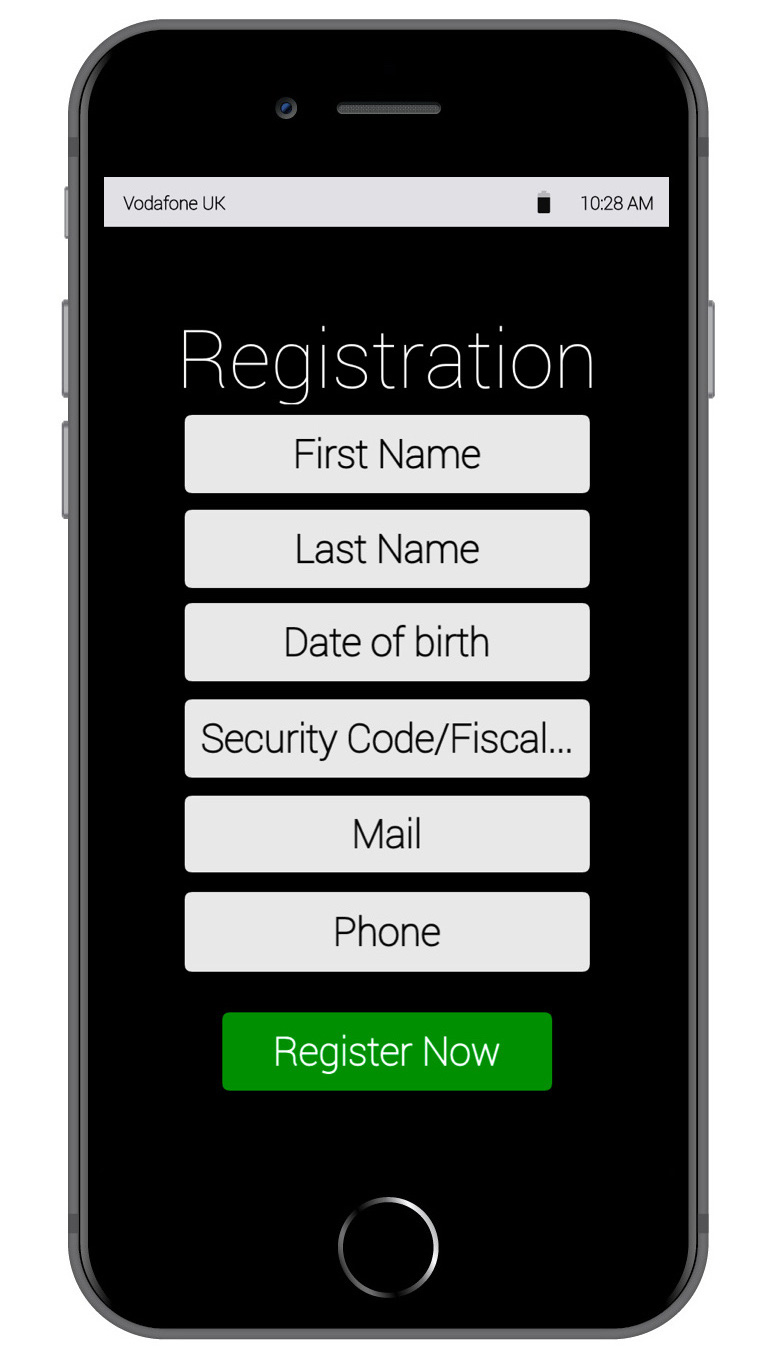
\includegraphics[height=14 cm]{Images/Mockups/Track4RunMockup4.jpg}
	\caption{Registration form.}
        \end{minipage}
      \end{center}
\end{figure}
In the first access to Track4Run App the user is asked to sign up or to sign in 			(Figure 2). Based on the fact that the user already has a TrackMe account or not will choose the right option. In future accesses to the App the user do not need to select each time one of these two possible options because the App automatically remembers the account which is logged in. In case of sign in (Figure 3), the user has to fill all the mandatory fields in order to complete the registration form. Once every field is correctly filled, it would be possible to complete the registration selecting the \textbf{Register Now} button. 
\clearpage
\begin{figure}[H]
\begin{center}
        \begin{minipage}[c]{.40\textwidth}
        \centering
          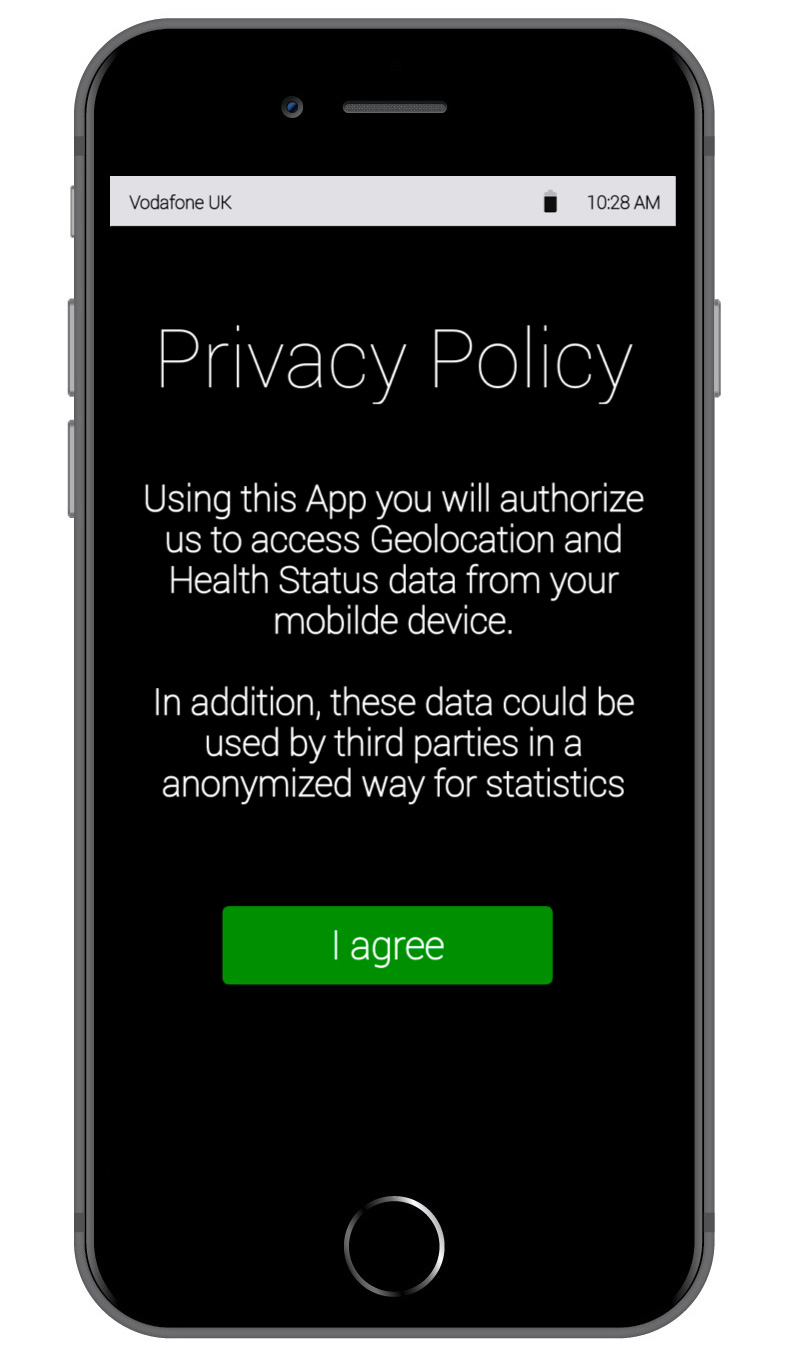
\includegraphics[height=14 cm]{Images/Mockups/Track4RunMockup2.jpg}
	\caption{Privacy Policy Conditions pt.1}
        \end{minipage}%
        \hspace{10mm}%
        \begin{minipage}[c]{.40\textwidth}
        \centering
          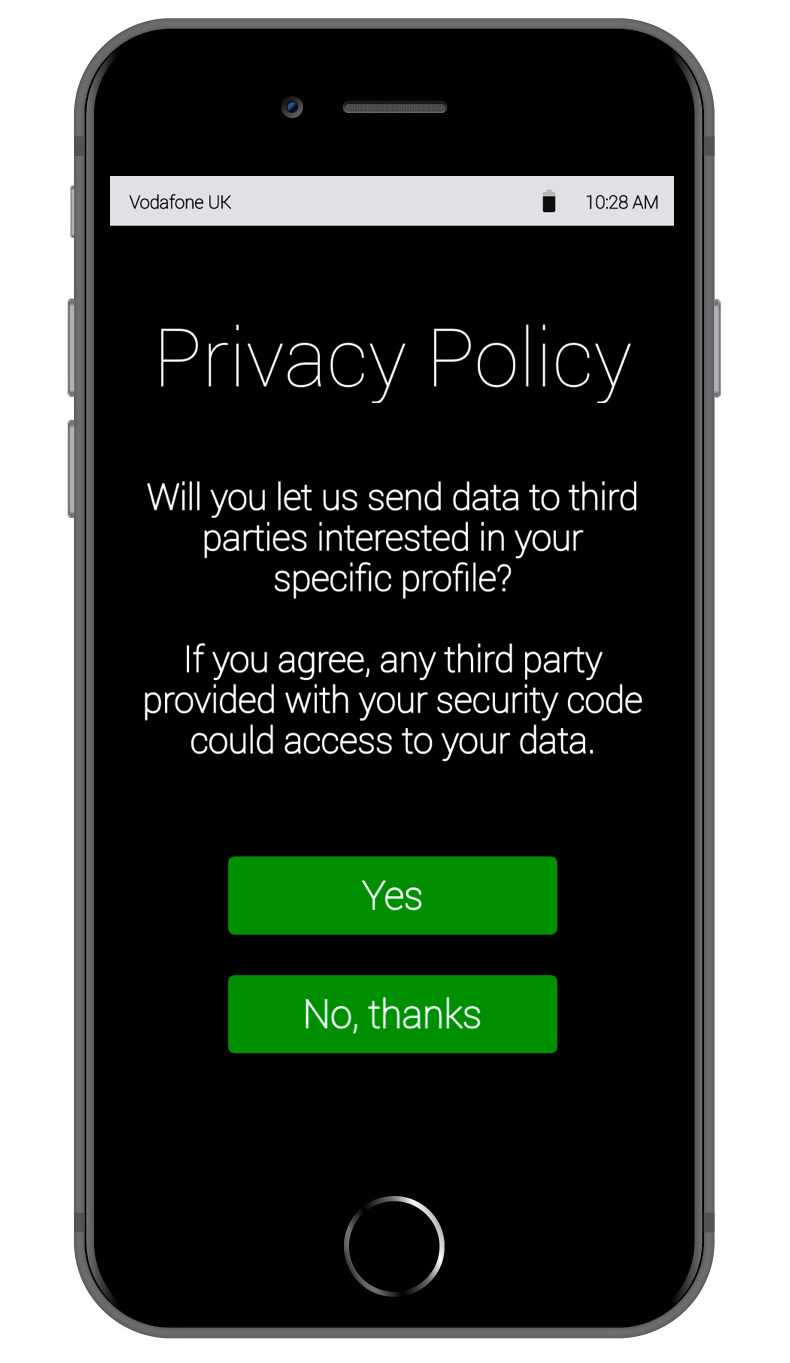
\includegraphics[height=14 cm]{Images/Mockups/Track4RunMockup3.jpg}
	\caption{Privacy Policy Conditions pt.2}
        \end{minipage}
      \end{center}
\end{figure}
During the first access to the App, the next step after sign up/sign in is to agree to the Privacy Policy Conditions (Figure 4). In order to use this App the user has to agree to the treatment of Location and Health Status data by Data4Help. In addition, these data could be used by third parties for the group monitoring request. Without agreeing the Privacy Policy Conditions the user can not go to the next page, therefore he/she will not be able to use this App. All the three first steps presented so far are substantially the same of AutomatedSOS. The next step regards the second part of the Privacy Policy Conditions (which was not presented for the previous system) about individual monitoring request (Figure 9).  In this case it is not strictly necessary to accept it, the user simply can select the \textbf{No, thanks} option.
\clearpage
\begin{figure}[H]
\begin{center}
        \begin{minipage}[c]{.40\textwidth}
        \centering
          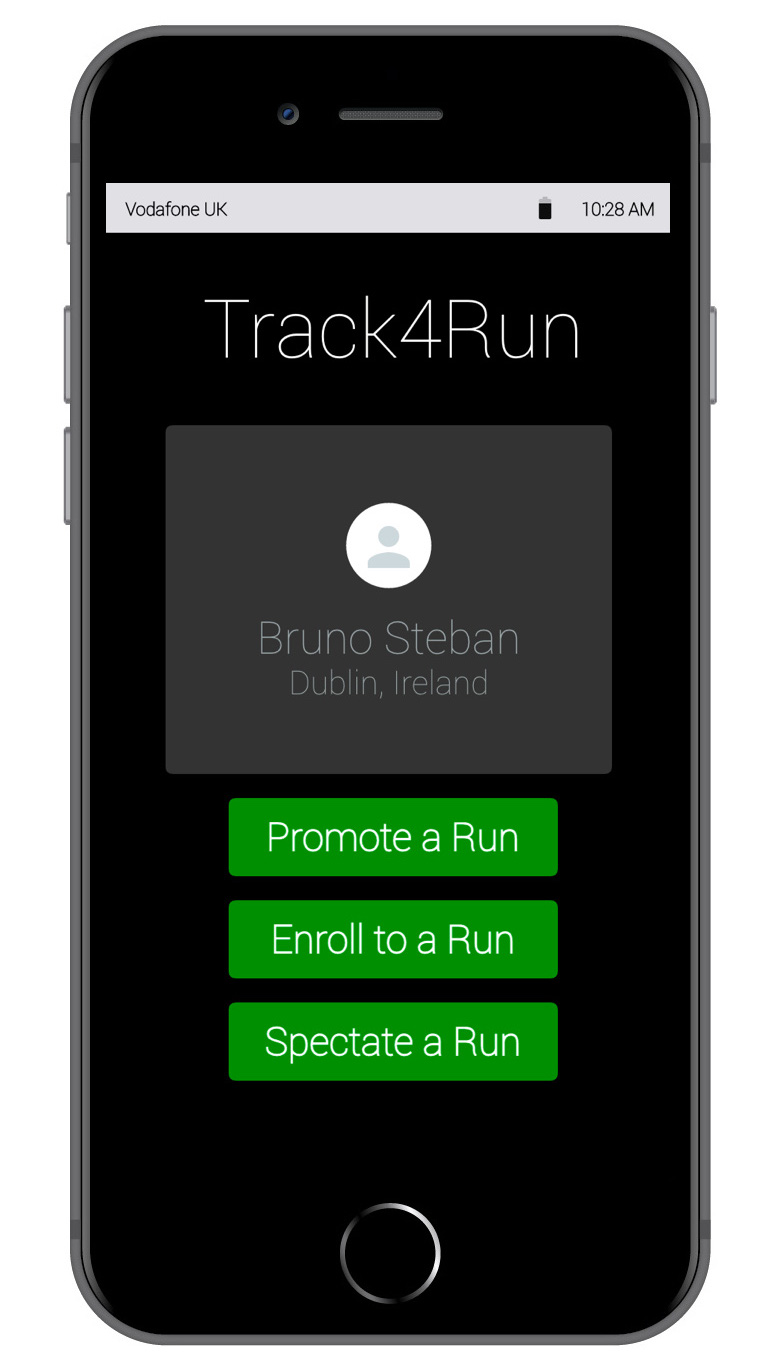
\includegraphics[height=14 cm]{Images/Mockups/Track4RunMockup5.jpg}
	\caption{Main menu.}
        \end{minipage}%
        \hspace{10mm}%
        \begin{minipage}[c]{.40\textwidth}
        \centering
          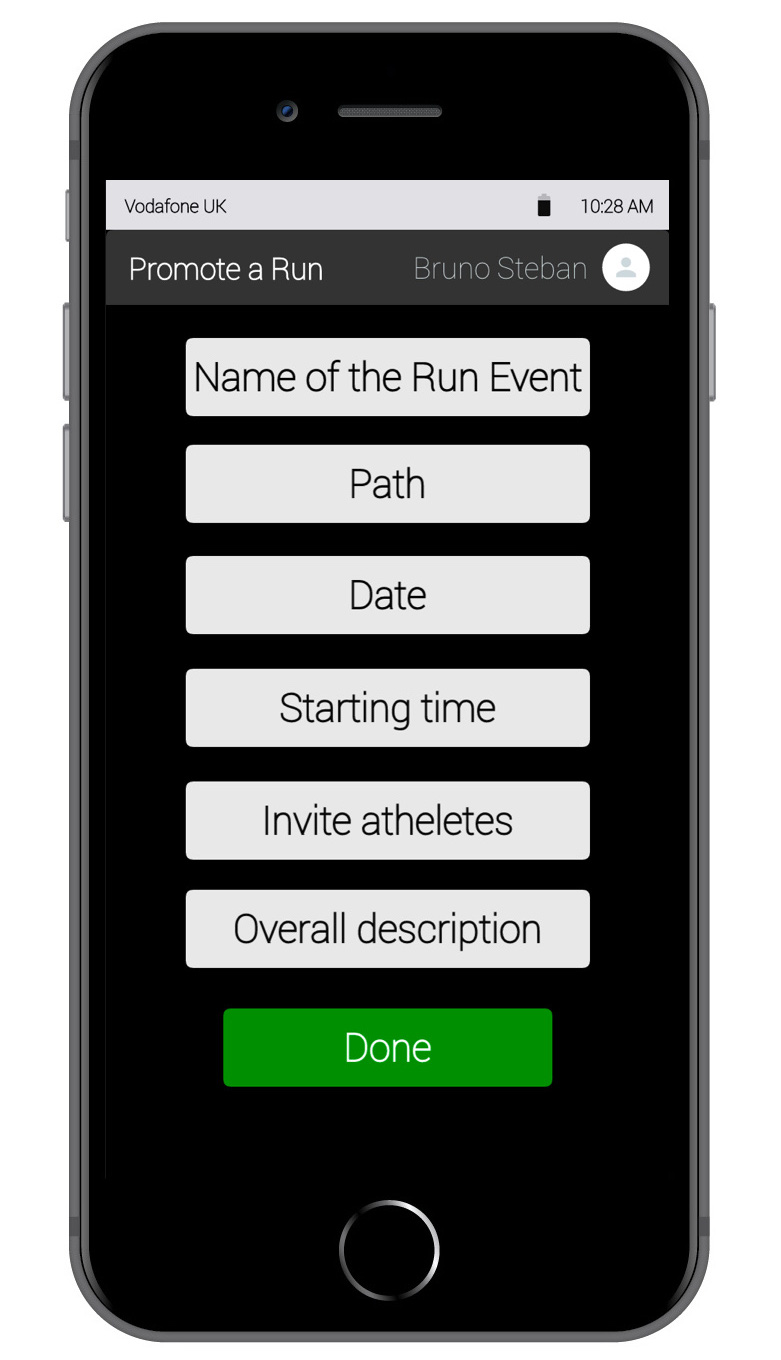
\includegraphics[height=14 cm]{Images/Mockups/Track4RunMockup6.jpg}
	\caption{Pomote a run view.}
        \end{minipage}
      \end{center}
\end{figure}
In Track4Run Home three options are possible. Selecting the first one, \textbf{Promote a Run}, a user can create a run event and promote it inviting athletes. The second option, which is \textbf{Enroll to a Run} allows the user enrol to a run. Finally, choosing \textbf{Spectate a Run} a spectator can see on a map the position of all runners during the run. Now, we analyze these three possibilities in detail. Choosing the first one the App leads the user to a new page in order to manage the event (Figure X). Here, it is possible to set all the necessary features of the run, like to define the path on a map, set the date, the starting time and so on. It is also possible to invite athletes to the run in order to promote the event.
\clearpage
\begin{figure}[H]
\begin{center}
        \begin{minipage}[c]{.40\textwidth}
        \centering
          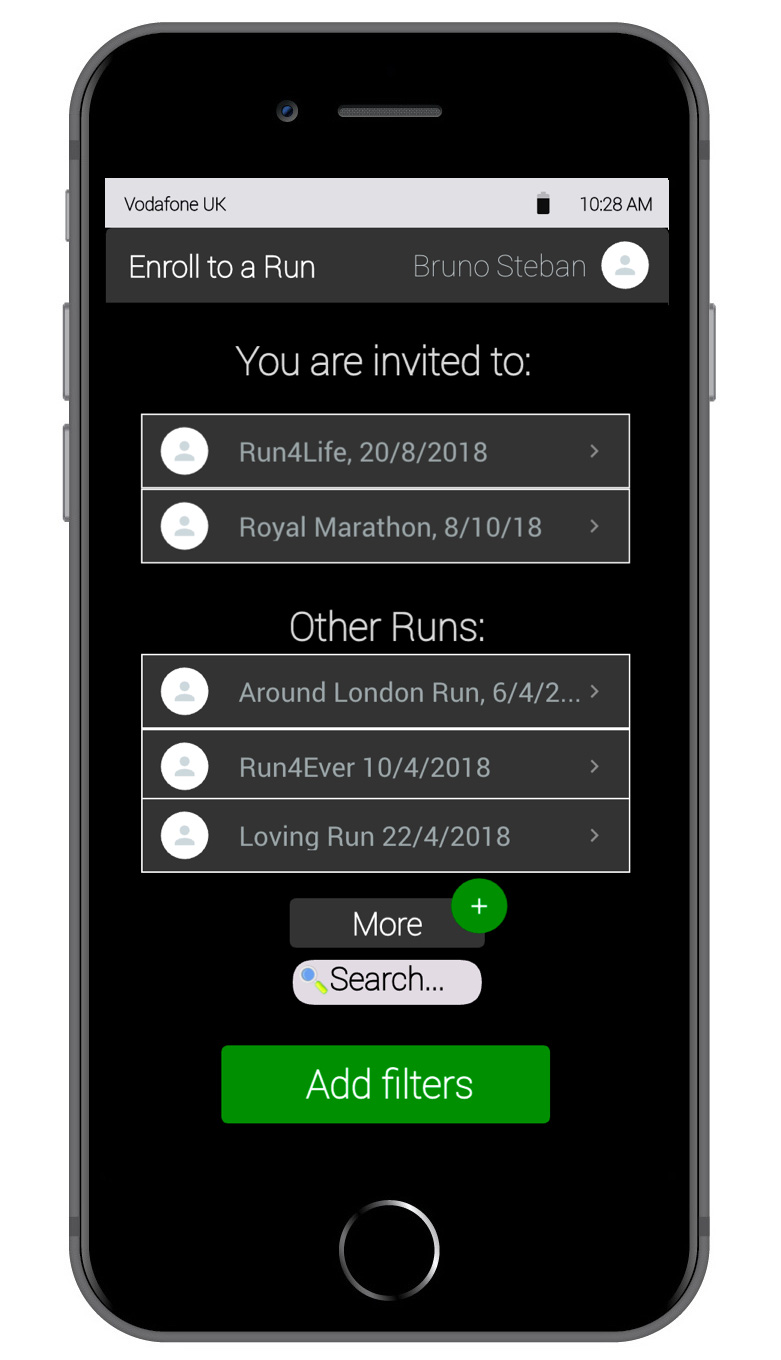
\includegraphics[height=14 cm]{Images/Mockups/Track4RunMockup7.jpg}
	\caption{Enroll to a run.}
        \end{minipage}%
        \hspace{10mm}%
        \begin{minipage}[c]{.40\textwidth}
        \centering
          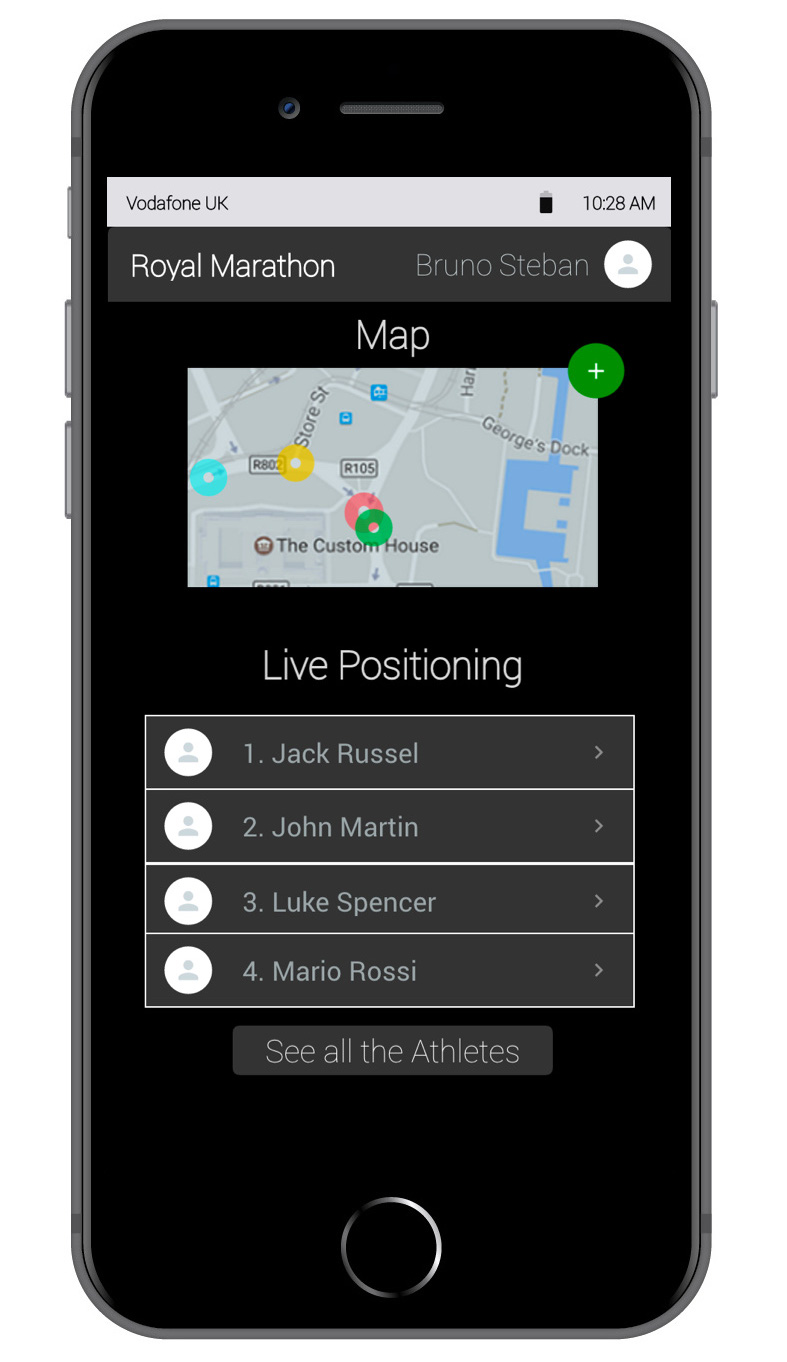
\includegraphics[height=14 cm]{Images/Mockups/Track4RunMockup8.jpg}
	\caption{Spectate a run view}.
        \end{minipage}
      \end{center}
\end{figure}
In the section Enroll to a Run (Figure X) a user can see a list of all the runs in which he/she has been invited. The user can select each of these runs to see furthermore details about it and at the end to enroll to it. A list of all the runs that will be soon held is showed immediately below. Since the large number of all the future runs, only a little portion of them is showed, selecting the \textbf{More +} button the user can see another set of run events. In addition, through \textbf{Add filters} it is possible to limit the list of the all runs to a spefic date, location and similar options. To easily access to a specific run, the \textbf{Search} button allows the user to immediately find the run he/she was looking for. In the last section, Spectate a Run (Figure X), it is possible to spectate to a specific run in a interactive way. A map shows all the runners enrolled in it, each one represented by a different coloured circle. Selecting the \textbf{+} button is possible to zoom in the map that will appear on full-screen mode. Below the map the live positioning show the first four athletes, anyway selecting \textbf{See all the Athletes} option it is possible to see the live positions of all the participants.
\clearpage
\end{enumerate}